\chapter{Support Vector Machines}
In this chapter, we will explore what are known as a support vector machines, or SVMs for short. SVMs are broadly useful for problems in classification and regression, and they are part of a family of techniques known as \textit{margin methods}. The defining goal of margin methods, and SVMs specifically, is to put as much distance as possible between data points and decision boundaries. We will dig deeper into what exactly this means over the course of the chapter. One of the most appealing aspects of SVMs is that they decompose into convex optimization problems, for which we can find a global optimum with relative ease. We will explore the mathematical underpinnings of SVMs, which can be slightly more challenging than our previous topics, as well as their typical use cases.

\section{Motivation}
While SVMs can be used for classification or regression, we will reason about them in the classification case as it is more straightforward. 

The grand idea behind SVMs is that we should construct a linear hyperplane in our feature space that maximally separates our classes, which means that the different classes should be as far from that hyperplane as possible. The distance of our data from the hyperplane is known as \textit{margin}.

\begin{definition}{Margin}{definition}
Margin is the distance of the nearest data point from the separating hyperplane of an SVM model, as seen in Figure \ref{fig:2d-hyperplane}. Larger margins often lead to more generalizable models.
\end{definition}

A larger margin tends to mean that our model will generalize better, since it provides more wiggle room to correctly classify unseen data.

\begin{figure}
    \centering
    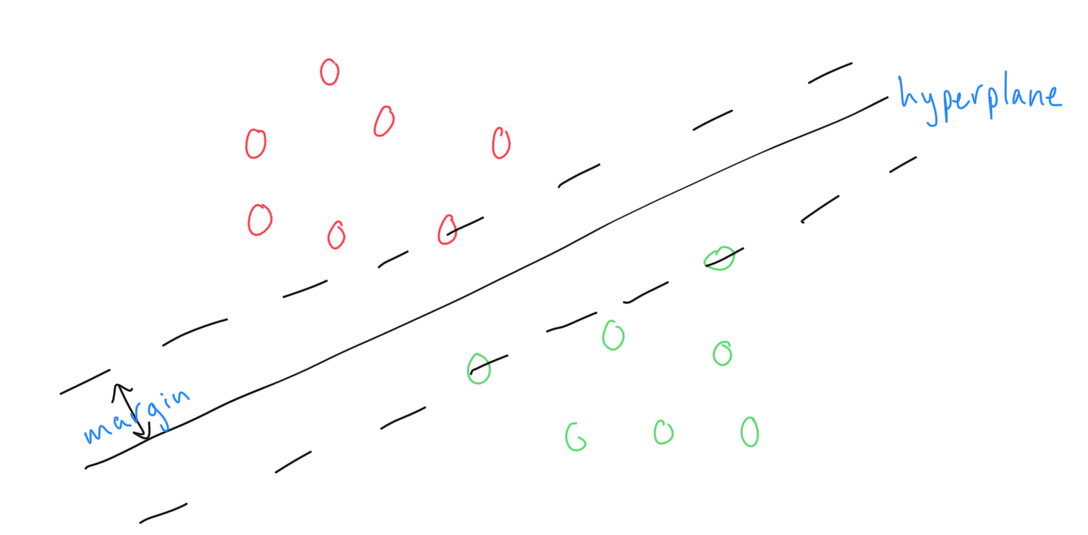
\includegraphics[width=0.5\paperwidth]{../SupportVectorMachines/fig/2d-hyperplane.png}
    \caption{Hyperplane with margin between different classes.}
    \label{fig:2d-hyperplane}
\end{figure}

This idea of margin is quite intuitive for humans. If you were presented with Figure \ref{fig:2d-hyperplane} and were asked to separate the two classes, you would likely draw the line that keeps data points as far from it as possible. SVMs and other margin-based methods will attempt to algorithmically recreate this intuition.

\subsection{Max Margin Methods}
SVMs are a specific instance of a broader class of model known as \textit{max margin methods}. Their name describes them well: they deal with creating a maximum margin between training data and decision boundary, with the idea that this leads to model generalizability. 

Other max margin methods are outside the scope of this textbook. Note that these alternative methods typically differ from SVMs in some non-trivial manner. For example, SVMs do not produce posterior probability distributions but rather decision rules for handling new data points. If you needed posterior probabilities for your model, there are other max margin methods better suited to that task.

\begin{mlcube}{Support Vector Machines}
SVMs are typically used in settings with discrete outputs. We need labeled training data to identify the relevant hyperplane in an SVM model. Finally, SVMs operate in a non-probabilistic setting.
\begin{center}
    \begin{tabular}{c|c|c}
    \textit{\textbf{Domain}} & \textit{\textbf{Training}} & \textit{\textbf{Probabilistic}} \\
    \hline
    Discrete & Supervised & No \\
    \end{tabular}
\end{center}
\end{mlcube}

\subsection{Applications}
The theory behind SVMs has been around for quite some time (since 1963), and prior to the rise of neural networks and other more computationally intensive techniques, SVMs were used quite extensively for image recognition, object categorization, and other typical machine learning tasks.

In particular, SVMs were and still are widely used for a subset of classification problems known as anomaly detection.
\readernote{The purpose of anomaly detection is to identify unusual data points. For example, if we are manufacturing widgets, we may wish to inspect and flag any widget that seems atypical with respect to the rest of the widgets we produce.}
Anomaly detection can be as simple as a binary classification problem where the data set is comprised of anomalous and non-anomalous data points. As we will see, an SVM can be constructed from this data set to identify future anomalous points very efficiently. SVMs continue to be competitive in many real-world situations where we can define good features for our data.

\section{Hard Margin Classifier for Linearly Separable Data}
We will learn the theory behind SVMs by starting with a simple two-class classification problem, as we've seen several times in previous chapters. We will constrain the problem even further by assuming that the two classes are linearly separable, which is the basis of the \textit{hard margin} formulation for SVMs.

\readernote{The expression `hard margin' simply means that we don't allow any data to be classified incorrectly. If it's not possible to find a hyperplane that perfectly separates the data based on class, then the hard margin classifier will return no solution.}

\subsection{Why the Hard Margin}
The hard margin constraint, which assumes that our data is linearly separable, is not actually a requirement for constructing an SVM, but it simplifies the problem initially and makes our derivations significantly easier. After we've established the hard margin formulation, we will extend the technique to work in situations where our data is not linearly separable.

\subsection{Deriving our Optimization Problem}
Recall that our goal is to define a hyperplane that separates our data points and maintains the maximum possible distance between the hyperplane and nearest data points on either side of it. To uncover this hyperplane, we start with a simple linear model for a two-class classification problem:
\begin{equation} \label{classification-fn}
f(\textbf{x}) = \textbf{w}^{T}\phi(\textbf{x}) + w_{0}
\end{equation}
where we have $N$ multidimensional data points $\textbf{x}_{1}, ..., \textbf{x}_{N}$, $\phi(\cdot)$ is a standard basis transformation function, and there is a bias term $w_{0}$. Each of our data point has a class $y_{1}, ..., y_{N}$ which is either $1$ or $-1$, and we assign new data points to class $1$ or $-1$ according to the sign produced by our trained model $f(\textbf{x})$.

By specifying our model this way, we have implicity defined a hyperplane separating our two classes given by:
\begin{equation} \label{implicit-hyperplane}
	\textbf{w}^{T}\phi(\textbf{x}) + w_{0} = 0
\end{equation}
Furthermore, we have that $\textbf{w}$ is orthogonal to the hyperplane, which we demonstrate now:

\begin{derivation}{Hyperplane Orthogonal to $\textbf{w}$}{hyperplane-derivation}
	Imagine two data points $x_{1}$ and $x_{2}$ on the hyperplane defined by $\textbf{w}^{T}\phi(\textbf{x}) + w_{0} = 0$. When we project their difference onto our model $\textbf{w}$, we find:
	\begin{equation} \label{hyperplane-eqn}
		\textbf{w}^{T}(\textbf{x}_{1} - \textbf{x}_{2}) = \textbf{w}^{T}\textbf{x}_{1} - \textbf{w}^{T}\textbf{x}_{2} = -w_{0} - (-w_{0}) = 0
	\end{equation}
	which means that $\textbf{w}$ is orthogonal to our hyperplane. We can visualize this in Figure \ref{fig:orthogonal-w}.
\end{derivation}

\begin{figure}
    \centering
    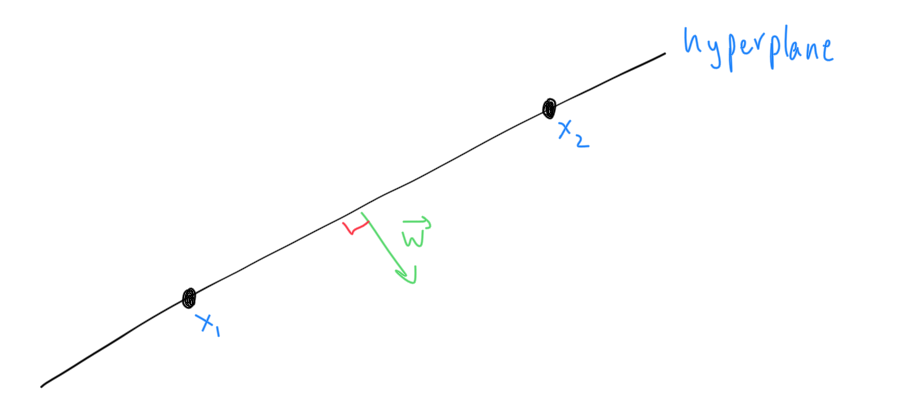
\includegraphics[width=0.5\paperwidth]{../SupportVectorMachines/fig/orthogonal-w.png}
    \caption{Our weight vector \textbf{w} is orthogonal to the separating hyperplane.}
    \label{fig:orthogonal-w}
\end{figure}

Remember that we're trying to maximize the margin between our training data and the hyperplane. The fact that $\textbf{w}$ is orthogonal to our hyperplane will help with this.

To determine the distance between a data point $\textbf{x}$ and the hyperplane, which we denote $d$, we need the distance in the direction of $\textbf{w}$ between the point and the hyperplane. We denote $\textbf{x}_{\perp}$ to be the projection of $\textbf{x}$ onto the hyperplane, which allows us to decompose $\textbf{x}$ as the following:
\begin{equation} \label{decompose-x}
	\textbf{x} = \textbf{x}_{\perp} + d \frac{\textbf{w}}{|| \textbf{w} ||}
\end{equation}
which is simply the sum of the portion of $\textbf{x}$ perpendicular to $\textbf{w}$ and the portion of $\textbf{x}$ that is parallel to $\textbf{w}$. From here we can solve for $d$:
\begin{derivation}{Distance from Hyperplane Derivation}{distance-from-hyperplane-derivation}
	We start by left multiplying Equation \ref{decompose-x} with $\textbf{w}^{T}$.
	\begin{align*}
		\textbf{w}^{T}\textbf{x} = \textbf{w}^{T}\textbf{x}_{\perp} + d \frac{\textbf{w}^{T}\textbf{w}}{||\textbf{w}||}
	\end{align*}
	Simplifying (note that $\textbf{w}^{T}\textbf{x}_{\perp} = -w_{0}$ from Equation \ref{hyperplane-eqn}):
	\begin{align*}
		\textbf{w}^{T}\textbf{x} =  - w_{0} + d ||\textbf{w}||
	\end{align*}
	Rearranging:
	\begin{align*}
		d = \frac{\textbf{w}^{T}\textbf{x} + w_{0}}{||\textbf{w}||}
	\end{align*}
\end{derivation}
which means that for each data point $\textbf{x}$, we now have the signed distance of that data point from the hyperplane.

To classify a data point correctly, the distance $d$ should be positive for class $y = 1$, and $d$ should be negative for class $y = -1$. For training purposes, we can make the margin positive whenever we correctly classify data by multiplying $y$ and $d$. Then, the margin for an individual data point $\textbf{x}_{n}$ is given by:
\begin{equation} \label{individual-margin}
	\frac{y_{n}(\textbf{w}^{T}\textbf{x}_{n} + w_{0})}{||\textbf{w}||}
\end{equation}
The margin for an entire data set is given by the margin to the closest point in the data set, given by:
\begin{equation} \label{total-margin}
	\min_{n} \frac{y_{n}(\textbf{w}^{T}\textbf{x}_{n} + w_{0})}{||\textbf{w}||}
\end{equation}
Then, it is our goal to maximize this margin with respect to our model parameters $\textbf{w}$ and $w_{0}$. This is given by:
\begin{equation} \label{total-maximized-margin}
	\underset{\textbf{w}, w_{0}}{\arg\max} \big\{ \frac{1}{||\textbf{w}||} \min_{n} y_{n}(\textbf{w}^{T}\textbf{x}_{n} + w_{0}) \big\}
\end{equation}
This is a hard problem to optimize, but we can make it more tractable by recognizing some important features of Equation \ref{total-maximized-margin}. First, rescaling $\textbf{w} \rightarrow \alpha \textbf{w}$ and $w_{0} \rightarrow \beta w_{0}$ has no impact on the relative distance of any data point $\textbf{x}_{n}$ from the hyperplane. We can use this rescaling liberty to enforce
\begin{equation} \label{enfore-dist-to-1}
	y_{n}(\textbf{w}^{T}\textbf{x}_{n} + w_{0}) = 1 \quad n, \text{closest}
\end{equation}
for the data point closest to the hyperplane. Thus, all of our data points have a margin that is greater than or equal to 1:
\begin{equation} \label{new-margin-constraint}
	\forall n \, y_{n}(\textbf{w}^{T}\textbf{x}_{n} + w_{0}) \geq 1 \quad n, \text{farther}
\end{equation}
which is used as a constraint in the optimization problem of Equation \ref{total-maximized-margin}. Thus our optimization problem now looks like:
\begin{equation} \label{simplified-maximized-margin-optimization}
	\underset{\textbf{w}, w_{0}}{\arg\max} \frac{1}{||\textbf{w}||} \quad \text{s.t.} \quad \forall n \, y_{n}(\textbf{w}^{T}\textbf{x}_{n} + w_{0}) \geq 1
\end{equation}
Notice that maximizing $\frac{1}{||\textbf{w}||}$ is equivalent to minimizing $||\textbf{w}||^{2}$. We will also add a constant term $\frac{1}{2}$ for convenience, leaving our final optimization problem:
\begin{equation} \label{final-simplified-maximized-margin-optimization}
	\underset{\textbf{w}, w_{0}}{\arg\min} \frac{1}{2} ||\textbf{w}||^{2} \quad \text{s.t.} \quad \forall n \, y_{n}(\textbf{w}^{T}\textbf{x}_{n} + w_{0}) \geq 1
\end{equation}
Note that Equation \ref{final-simplified-maximized-margin-optimization} is now a quadratic programming problem, which means we wish to optimize a quadratic function subject to a set of linear constraints on our parameters. Arriving at this form was the motivation for the preceding mathematic manipulations. We will discuss shortly how we actually optimize this function.

\subsection{What is a Support Vector}
Up until now, we have discussed Support Vector Machines without identifying what a support vector is. We now have enough information from the previous section to define them.

\begin{definition}{Support Vector}{support-vector}
The support vectors in an SVM are the data points closest to the hyperplane.
\end{definition}

In the hard margin case we have constrained the closest data points to being a distance of 1 from the hyperplane, so the support vectors are all $d=1$ from the hyperplane. Figure \ref{fig:hard-margin-svm} shows a hard margin SVM solution with the corresponding support vectors.

\readernote{After we have optimized an SVM in the hard margin case, we must have at least two support vectors with a distance of 1 from the hyperplane.}

\begin{figure}
    \centering
    \textbf{Hard Margin SVM Example}\par\medskip
    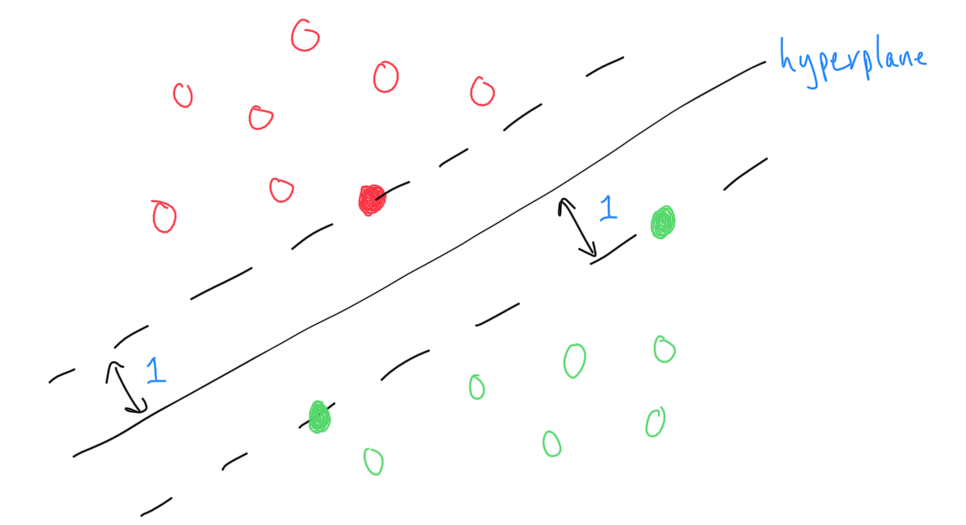
\includegraphics[width=0.5\paperwidth]{../SupportVectorMachines/fig/hard-margin-svm.png}
    \caption{Example of the resulting hyperplane for a hard margin SVM. The filled in data points are support vectors.}
    \label{fig:hard-margin-svm}
\end{figure}

\section{Soft Margin Classifier}
Thus far, we've been operating under the assumption that our data is linearly separable in feature space, which afforded us several convenient guarantees in the derivations of the previous section. For example, given that our data was linearly separable, we could guarantee that every data point would be on the correct side of the hyperplane, which was part of what allowed us to enforce the constraint that $d=1$ for the points closest to the hyperplane. We now seek to generalize the work of the previous section to situations where our data is not so nice.

\subsection{Why the Soft Margin?}
What if our data is not linearly separable in transformed feature space? For a real, complex problem domain, it's highly unlikely that it would be. Unfortunately, our current hard margin SVM formulation would be useless with non-linearly separable data. That is why we need the soft margin SVM.

\begin{figure}
    \centering
    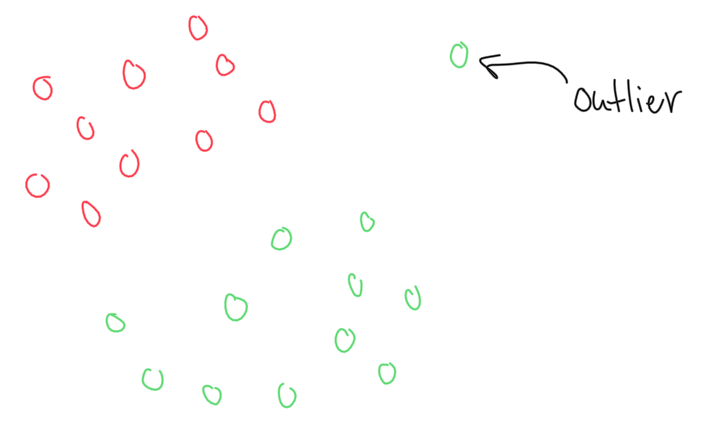
\includegraphics[width=0.5\paperwidth]{../SupportVectorMachines/fig/outlier-data-pt.png}
    \caption{An outlier can make the hard margin formulation impossible or unable to generalize well.}
    \label{fig:outlier-data-pt}
\end{figure}

At a high level, the soft margin SVM allows for some of our data points to be closer to or even on the incorrect side of the hyperplane. This is desirable if our data set is not linearly separable or contains outliers, and it is also quite intuitive. Examining Figure \ref{fig:outlier-data-pt}, we see that we have a single outlier data point. We can still create a good model by just allowing this single data point to be close to the hyperplane. That is what the soft margin formulation will allow for.

\subsection{Updated Optimization Problem for Soft Margins}
To enable the soft margin formulation, we introduce what are known as \textit{slack variables} denoted $\xi_{n} \geq 0$, which simply relax the constraint from Equation \ref{new-margin-constraint} that we imposed in the hard margin formulation. There is a slack variable $\xi_{n} \geq 0$ for every data point $\textbf{x}_{n}$, and they take the following values according to how we classify $\textbf{x}_{n}$:
\begin{equation} \label{slack-variable-values}
	\xi_{n} = \begin{cases}
	 	= 0 & \text{if correctly classified} \\
		\in (0, 1] & \text{if correctly classified but inside margin} \\
		> 1 & \text{if incorrectly classified} \\
	\end{cases}
\end{equation}
These slack variable penalize data points on the wrong side of the margin defined by the hyperplane, but they don't forbid us from allowing data points to be on the wrong side if it produces the best model. We now reformulate our optimization problem as:
\begin{equation} \label{soft-margin-optimization-problem}
	\underset{\textbf{w}, w_{0}}{\arg\min} \frac{1}{2} ||\textbf{w}||^{2} + C \sum_{n=1}^{N} \xi_{n} \quad \text{s.t.} \quad \forall n \, y_{n}(\textbf{w}^{T}\textbf{x}_{n} + w_{0}) \geq 1 - \xi_{n}, \quad \xi_{n} \geq 0
\end{equation}
where $C$ is a regularization parameter that determines how heavily we penalize violations of the hard margin constraints. A large $C$ penalizes violation of the hard margin constraints more heavily, which means our model will follow the data closely and have little regularization. A small $C$ won't heavily penalize having data points inside the margin region, relaxing the constraint and allowing our model to somewhat disregard more of the data. This means more regularization.

\readernote{Unlike most regularization parameters we've seen thus far, $C$ increases regularization as it gets smaller.}

\subsection{Soft Margin Support Vectors}
Under the the hard margin formulation, the support vectors were those data points exactly $d=1$ from the hyperplane, and they were also guaranteed to be the points closest to the hyperplane. Under the soft margin formulation, we no longer have this guarantee since we explicity relaxed it in the name of creating better, more generalizable models.

The support vectors for the soft margin case are determined by the value of the slack variable $\xi_{n}$ defined in Equation \ref{slack-variable-values}: data points for which $\xi_{n} \geq 0$ are the support vectors. Note that these support vectors are either correctly classified but within/on the margin ($\xi_{n} \in [0,1]$) or incorrectly classified ($\xi_{n} > 1$). We can visualize this in Figure \ref{fig:soft-margin-svm}.

\readernote{Data points for which $\xi_{n} = 0$ are on the margin and are still considered support vectors.}

\begin{figure}
    \centering
    \textbf{Soft Margin SVM Example}\par\medskip
    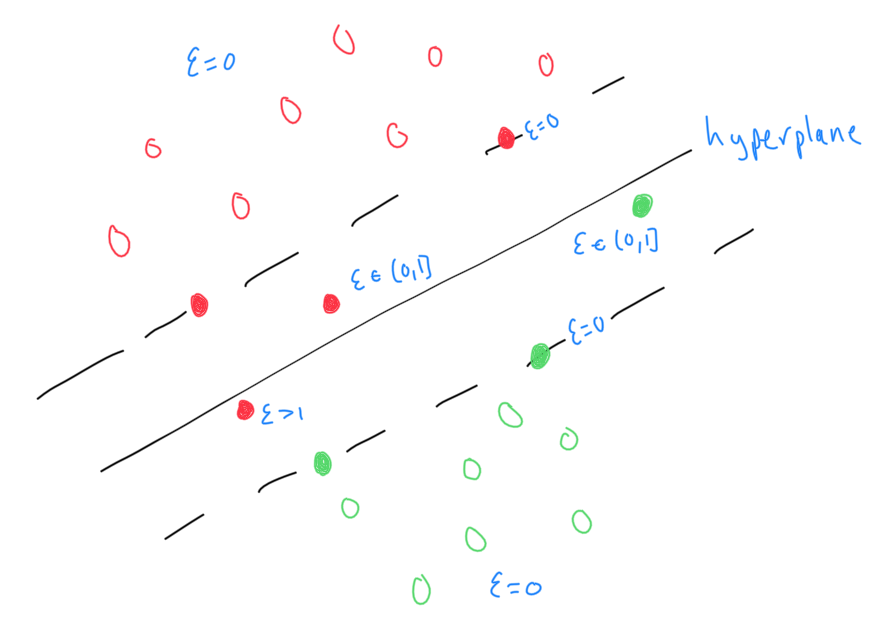
\includegraphics[width=0.5\paperwidth]{../SupportVectorMachines/fig/soft-margin-svm.png}
    \caption{Example of the resulting hyperplane for a soft margin SVM. The filled in data points are support vectors.}
    \label{fig:soft-margin-svm}
\end{figure}

\section{Conversion to Dual Form}
Now that we have the formulation of the optimization problem for SVMs, we need to discuss how we actually go about optimizing to produce a model solution. This will involve converting to a \textit{dual form} of our problem. We will do this in the hard margin case for notational simplicity, but our solution will apply to the soft margin formulation as well.

\readernote{A dual form is simply an equivalent manner of representing some expression, in this case the quadratic programming problem we need to optimize.}

\subsection{Lagrange Multipliers}
Before we get into deriving the dual form, we need to be aware of a critical piece of math that will enable us to solve our optimization problem: \textit{Langrange multipliers}.

A Lagrange multiplier is used to find optima of a function subject to certain constraints. This is exactly what we need to solve the optimization problem described by Equation \ref{final-simplified-maximized-margin-optimization}.

The underlying theory behind Lagrange multipliers is not overly difficult to understand, but it is beyond the scope of this textbook. We will simply offer the method by which you can use them to solve optimization problems.

If you have a function $f(\textbf{x})$ which you need to optimize (let's say maximization here to be concrete, but minimization applies just the same) subject to the constraint that some function $g(\textbf{x}) = 0$, you can take the following steps. First, construct the Lagrangian function $L(\textbf{x}, \lambda)$:
\begin{equation} \label{lagrangian-fn}
	L(\textbf{x}, \lambda) = f(\textbf{x}) + \lambda g(\textbf{x})
\end{equation}
Then, set the derivative of $L$ with respect to both $\textbf{x}$ and $\lambda$ equal to 0:
\begin{equation*}
	\nabla L_{\textbf{x}} = 0, \qquad \frac{\partial L}{\partial \lambda} = g(\textbf{x}) = 0
\end{equation*}
If $\textbf{x}$ is $D$-dimensional, this will give you a system of $D+1$ equations. You can solve these equations for $\textbf{x}$ to find the optimal value of $f(\textbf{x})$ subject to the constraint $g(\textbf{x})$.

You should also be aware of the case where your constraint $g(\textbf{x})$ is an inequality. If we have $g(\textbf{x}) \geq 0$, we will still have the Lagrangian function given by Equation \ref{lagrangian-fn}. On the other hand, if the inequality constraint is $g(\textbf{x}) \leq 0$, construct your Lagrangian function as follows:
\begin{equation*}
	L(\textbf{x}, \lambda) = f(\textbf{x}) - \lambda g(\textbf{x})
\end{equation*}
where only the sign has changed between the $f(\textbf{x})$ and $g(\textbf{x})$ terms. We will work in the $g(\textbf{x}) \geq 0$ case, which like before we optimize with respect to the parameters $\textbf{x}$ and $\lambda$:
\begin{equation*}
	\nabla L_{\textbf{x}} = 0, \qquad \frac{\partial L}{\partial \lambda} = g(\textbf{x}) \geq 0
\end{equation*}
Regardless of the direction of the inequality, we also now optimize subject to the constraints:
\begin{equation*}
	\qquad \lambda \geq 0, \qquad \lambda g(\textbf{x}) = 0
\end{equation*}

\readernote{The exact reason for these new constraints when working with inequalities is beyond the scope of this textbook, but it's important to remember that they be met.}

Finally, note that when you are optimizing a function under many constraints, you simply introduce a Lagrange multiplier for each constraint.

\begin{example}{Langrange Multiplier Example}{lagrange-multiplier-example}
	Let's say we had a function $f(\textbf{x})$ we wish to maximize:
	\begin{align*}
		f(\textbf{x}) = x_{1}^{2} + 3x_{2}^{2} + 3
	\end{align*}
	subject to the constraint $g(\textbf{x})$:
	\begin{align*}
		g(\textbf{x}) = 4x_{1} + 4x_{2} - 6 = 0
	\end{align*}
	We begin by construction our Lagrangian function $L(\textbf{x}, \lambda)$:
	\begin{align*}
		L(\textbf{x}, \lambda) = x_{1}^{2} + 3x_{2}^{2} + 3 + \lambda (4x_{1} + 4x_{2} - 6)
	\end{align*}
	We then compute $\nabla L_{\textbf{x}}$ and $\frac{\partial L}{\partial \lambda}$ to get a system of equations:
	\begin{align*}
		2x_{1} + 4\lambda = 0 \\
		6x_{2} + 4\lambda = 0 \\
		4x_{1} + 4x_{2} - 6 = 0
	\end{align*}
	Solving these equations for $x_{1}$, $x_{2}$, and $\lambda$ leaves us with the following mazimized solution:
	\begin{align*}
		(x_{1}^{*}, x_{2}^{*}) = \bigg(\frac{9}{8}, \frac{3}{8}\bigg); \qquad \lambda^{*} = -\frac{9}{16}
	\end{align*}
\end{example}

\subsection{Deriving the Dual Formulation}
Now that we understand Lagrange multipliers and how we can use them for constrained optimization, we can get back to the hard margin SVM optimization problem:
\begin{equation} \label{original-optim-fn}
	\underset{\textbf{w}, w_{0}}{\arg\min} \frac{1}{2} ||\textbf{w}||^{2} \quad \text{s.t.} \quad \forall n \, y_{n}(\textbf{w}^{T}\textbf{x}_{n} + w_{0}) \geq 1
\end{equation}
To satisfy these $N$ constraints, we introduce $N$ Lagrange multipliers $\lambda_{0}, ..., \lambda_{N-1} \geq 0$. We then have our Lagrangian function:
\begin{equation} \label{lagrange-equation}
	L(\textbf{w}, w_{0}, \boldsymbol{\lambda}) = \frac{1}{2} ||\textbf{w}||^{2} - \sum_{n=1}^{N} \lambda_{n} (y_{n}(\textbf{w}^{T} \textbf{x}_{n} + w_{0}) - 1)
\end{equation}
where $\boldsymbol{\lambda} = \lambda_{0}, ..., \lambda_{N-1}$. Using this Lagrangian function, we allow ourselves to switch from solving Equation \ref{original-optim-fn} to instead solving:
\begin{equation} \label{new-optim-fn}
	\underset{\textbf{w}, w_{0}}{\arg\min} \max_{\boldsymbol{\lambda} \geq 0} L(\textbf{w}, w_{0}, \boldsymbol{\lambda})
\end{equation}

\readernote{The `$\underset{\textbf{w}, w_{0}}{\arg\min} \, \underset{\boldsymbol{\lambda} \geq 0}{\max}$' in Equation \ref{new-optim-fn} may be initially confusing. We introduce the maximum because the values of $\boldsymbol{\lambda}$ are free and should be set such that $L(\textbf{w}, w_{0}, \boldsymbol{\lambda})$ is as large as possible prior to minimizing with respect to $\textbf{w}, w_{0}$.}

We now wish to convert the objective in Equation \ref{new-optim-fn} to a dual objective. Under the sufficient conditions of strong duality which hold for this problem but whose explanation is beyond the scope of this textbook, we can reformulate the objective as:
\begin{equation} \label{dual-objective}
	\max_{\boldsymbol{\lambda} \geq 0} \underset{\textbf{w}, w_{0}}{\arg\min} L(\textbf{w}, w_{0}, \boldsymbol{\lambda})
\end{equation}
At this point, we can solve for $\textbf{w}, w_{0}$. Taking the gradient, setting equal to 0, and solving for $\textbf{w}$:
\begin{align*}
	\nabla L_{\textbf{w}} = \textbf{w} - \sum_{n=1}^{N} \lambda_{n} y_{n} \textbf{x}_{n} = 0
\end{align*}
\begin{equation} \label{solve-for-w}
	\textbf{w}^{*} = \sum_{n=1}^{N} \lambda_{n} y_{n} \textbf{x}_{n}
\end{equation}
And now for $w_{0}$:
\begin{align*}
	\frac{\partial L}{\partial w_{0}} = - \sum_{n=1}^{N} \lambda_{n} y_{n} = 0
\end{align*}
\begin{equation} \label{solve-for-w0}
	\sum_{n=1}^{N} \lambda_{n} y_{n} = 0
\end{equation}
Now that we have these equations defining the optimal values for $\textbf{w}$ and $w_{0}$ we plug them back into our our Lagrangian function:
\begin{equation} \label{plugged-in-lagrangian}
	\begin{aligned}
		L(\textbf{w}, w_{0}, \boldsymbol{\lambda}) = \frac{1}{2} || \sum_{n=1}^{N} \lambda_{n} y_{n} \textbf{x}_{n} ||^{2} - \sum_{n=1}^{N} \lambda_{n} y_{n} (\sum_{m=1}^{N} \lambda_{m} y_{m} \textbf{x}_{m})^{T} \textbf{x}_{n} - \sum_{n=1}^{N} \lambda_{n} y_{n} w_{0} + \sum_{n=1}^{N} \lambda_{n} \\
		= \frac{1}{2} \sum_{n=1}^{N} \sum_{m=1}^{N} \lambda_{n} \lambda_{m} y_{n} y_{m} \textbf{x}_{n}^{T} \textbf{x}_{m} - \sum_{n=1}^{N} \sum_{m=1}^{N} \lambda_{n} \lambda_{m} y_{n} y_{m} \textbf{x}_{n}^{T} \textbf{x}_{m} - w_{0} \sum_{n=1}^{N} \lambda_{n} y_{n} + \sum_{n=1}^{N} \lambda_{n} \\
		= \sum_{n=1}^{N} \lambda_{n} - \frac{1}{2} \sum_{n=1}^{N} \sum_{m=1}^{N} \lambda_{n} \lambda_{m} y_{n} y_{m} \textbf{x}_{n}^{T} \textbf{x}_{m}
	\end{aligned}
\end{equation}
We're left with the result of Equation \ref{plugged-in-lagrangian}, which is another quadratic function that we wish to maximize subject to the constraint $\boldsymbol{\lambda} \geq 0$ and $\sum_{n=1}^{N} \lambda_{n} y_{n} = 0$. We can solve for $\boldsymbol{\lambda}$ using the same Langrangian techniques described above.

Why do we wish to solve for the values of $\boldsymbol{\lambda}$ at all? To see this, we need to understand how to make predictions on new data points.

\subsection{Making Predictions}
Recall the classification function described by Equation \ref{classification-fn} at the beginning of this chapter:
\begin{equation*}
f(\textbf{x}) = \textbf{w}^{T}\phi(\textbf{x}) + w_{0}
\end{equation*}
We classifying new data points by looking at the sign produced by this function. Now that we've solved for \textbf{w}, we can rewrite this function as:
\begin{equation} \label{new-classification-fn}
	f(\textbf{x}) = \sum_{n=1}^{N} \lambda_{n} y_{n} \phi(\textbf{x}_{n})^{T} \phi(\textbf{x}_{n}) + w_{0}
\end{equation}
Data points for which $f(\textbf{x}) > 0$ are classified as $1$, while all other data points are classified as $-1$. Remember also that since $\boldsymbol{\lambda}$ are Lagrange multipliers, we are bound by the constraints:
\begin{align*}
	\lambda_{n} \geq 0, \quad \lambda_{n} \{y_{n} f(\textbf{x}_{n}) - 1\} = 0
\end{align*}
which means that for every data point summed in the Equation \ref{new-classification-fn}, we either have that $\lambda_{n} = 0$ or $y_{n} f(\textbf{x}_{n}) = 1$. Any data points where $\lambda_{n} = 0$ don't appear in the summation and thus don't have any impact on the prediction.

The rest of the data points, for which $\lambda_{n} > 0$, are known as \textbf{support vectors}, and because we have that $y_{n} f(\textbf{x}_{n}) = 1$, these are the data points that lie on the margin of the hyperplane in Figure \ref{fig:soft-margin-svm}.

This is a major takeaway for the usefulness of SVMs: once we've trained our model, we can discard most of our data. We only need to keep the support vectors to make predictions. This also illustrates why we need to solve for the values of $\boldsymbol{\lambda}$: those values dictate which data points are the support vectors for our model.

Finally, note that the extension of this solution from the hard margin to the soft margin case is straightforward. In fact, the Lagrangian function ends up being identical and we only have a few extra constraints.

\subsection{Why is the Dual Formulation Necessary?}
At this point, you might be wondering what exactly we gained by moving to the dual formulation of this problem.

First, the complexity of the optimization problem we're solving changed from one that is dependent on the number of features $M$ in our particular data domain to one that is linearly dependent on the number of data points $N$. Thus, our model complexity is now independent of the dimensionality of the feature space.

Second, in the dual formulation, we have the opportunity to take advantage of what's known as the \textit{kernel trick} to map our data $\textbf{x}_{n}$ into higher dimensions without incurring performance costs. This works as follows: notice that during our training process and at prediction time through Equation \ref{new-classification-fn}, we have the term $\phi(\textbf{x}_{n})^{T} \phi(\textbf{x}_{m})$. We rewrite this as follows:
\begin{equation} \label{kernel-fn}
	k(\textbf{x}_{n}, \textbf{x}_{m}) = \phi(\textbf{x}_{n})^{T} \phi(\textbf{x}_{m})
\end{equation}
where $k(\textbf{x}_{n}, \textbf{x}_{m})$ is known as the kernel function. Under certain conditions, we can skip the step of projecting data points $\textbf{x}_{n}$ into the larger basis defined by the transformation $\phi$, instead directly computing the value of the kernel function. We can use this trick as long as $k()$ is a valid kernel, which we turn to next.

\readernote{This trick can even be used to work in an infinite basis. If that is of interest, you should look into Taylor series basis expansion.}

\subsection{Kernel Composition}
Now that we've seen the usefulness of the kernel trick for working in higher dimensional spaces without incurring performance costs or memory overhead, it's reasonable to wonder what sort of valid kernels we can construct.

To be explicit, by `kernel' we mean a function that produces a scalar product from two vectors in your desired feature space. In other words, when applied to two data points, your kernel should produce a number. Although it is beyond the scope of this textbook, the condition for a kernel $k(\cdot)$ to be valid is that the matrix of elements given by $k(\textbf{x}_{n}, \textbf{x}_{m})$ should be positive semidefinite for all choices of the data set $\{ \textbf{x}_{n} \}$.

\readernote{The matrix of elements $k(\textbf{x}_{n}, \textbf{x}_{m})$ is known as the \textit{Gram matrix}, and is denoted by $\textbf{K}$.}

In practice we care that we can compose valid kernels from smaller valid kernels. To this end, there exists a set of rules that will preserve the validity of kernels through transformations. These include such things as scalar multiplication \big($c \cdot k(\textbf{x}_{n}, \textbf{x}_{m})$\big), exponentiation \big($\exp{\{k(\textbf{x}_{n}, \textbf{x}_{m})\}}$\big), and addition \big($k_{1}(\textbf{x}_{n}, \textbf{x}_{m}) + k_{2}(\textbf{x}_{n}, \textbf{x}_{m})$\big) and multiplication \big($k_{1}(\textbf{x}_{n}, \textbf{x}_{m}) \cdot k_{2}(\textbf{x}_{n}, \textbf{x}_{m})$\big) of different kernels. It is always possible to test the validity of a given kernel by demonstrating that its Gram matrix $\textbf{K}$ is positive semidefinite.
